\documentclass[12pt,letterpaper]{article}
\usepackage{graphicx,textcomp}
\usepackage{natbib}
\usepackage{setspace}
\usepackage{fullpage}
\usepackage{color}
\usepackage[reqno]{amsmath}
\usepackage{amsthm}
\usepackage{fancyvrb}
\usepackage{amssymb,enumerate}
\usepackage[all]{xy}
\usepackage{endnotes}
\usepackage{lscape}
\newtheorem{com}{Comment}
\usepackage{float}
\usepackage{hyperref}
\newtheorem{lem} {Lemma}
\newtheorem{prop}{Proposition}
\newtheorem{thm}{Theorem}
\newtheorem{defn}{Definition}
\newtheorem{cor}{Corollary}
\newtheorem{obs}{Observation}
\usepackage[compact]{titlesec}
\usepackage{dcolumn}
\usepackage{tikz}
\usetikzlibrary{arrows}
\usepackage{multirow}
\usepackage{xcolor}
\newcolumntype{.}{D{.}{.}{-1}}
\newcolumntype{d}[1]{D{.}{.}{#1}}
\definecolor{light-gray}{gray}{0.65}
\usepackage{url}
\usepackage{listings}
\usepackage{color}

\definecolor{codegreen}{rgb}{0,0.6,0}
\definecolor{codegray}{rgb}{0.5,0.5,0.5}
\definecolor{codepurple}{rgb}{0.58,0,0.82}
\definecolor{backcolour}{rgb}{0.95,0.95,0.92}

\lstdefinestyle{mystyle}{
	backgroundcolor=\color{backcolour},   
	commentstyle=\color{codegreen},
	keywordstyle=\color{magenta},
	numberstyle=\tiny\color{codegray},
	stringstyle=\color{codepurple},
	basicstyle=\footnotesize,
	breakatwhitespace=false,         
	breaklines=true,                 
	captionpos=b,                    
	keepspaces=true,                 
	numbers=left,                    
	numbersep=5pt,                  
	showspaces=false,                
	showstringspaces=false,
	showtabs=false,                  
	tabsize=2
}
\lstset{style=mystyle}
\newcommand{\Sref}[1]{Section~\ref{#1}}
\newtheorem{hyp}{Hypothesis}

\title{Problem Set 2}
\date{Due: October 14, 2024}
\author{Applied Stats/Quant Methods 1}

\begin{document}
	\maketitle
	\section*{Instructions}
\begin{itemize}
	\item Please show your work! You may lose points by simply writing in the answer. If the problem requires you to execute commands in \texttt{R}, please include the code you used to get your answers. Please also include the \texttt{.R} file that contains your code. If you are not sure if work needs to be shown for a particular problem, please ask.
	\item Your homework should be submitted electronically on GitHub.
	\item This problem set is due before 23:59 on Monday October 14, 2024. No late assignments will be accepted.

\end{itemize}

\vspace{.5cm}
\section*{Question 1: Political Science}
\vspace{.25cm}
	The following table was created using the data from a study run in a major Latin American city.\footnote{Fried, Lagunes, and Venkataramani (2010). ``Corruption and Inequality at the Crossroad: A Multimethod Study of Bribery and Discrimination in Latin America. \textit{Latin American Research Review}. 45 (1): 76-97.} As part of the experimental treatment in the study, one employee of the research team was chosen to make illegal left turns across traffic to draw the attention of the police officers on shift. Two employee drivers were upper class, two were lower class drivers, and the identity of the driver was randomly assigned per encounter. The researchers were interested in whether officers were more or less likely to solicit a bribe from drivers depending on their class (officers use phrases like, ``We can solve this the easy way'' to draw a bribe). The table below shows the resulting data.

\newpage
	\begin{table}[h!]
		\centering
		\begin{tabular}{l | c c c }
			& Not Stopped & Bribe Requested & Stopped/Given Warning \\ \hline
			Upper class & 14 & 6 & 7 \\
			Lower class & 7 & 7 & 1 \\ \hline
		\end{tabular}
		\caption{Police encounters by class and type of action}
	\end{table}
\begin{enumerate}
	
	\item [(a)]
	Calculate the $\chi^2$ test statistic by hand/manually (even better if you can do "by hand" in \texttt{R}).\\
	\begin{itemize}
		\item Assumption:
		\newline
		\item Random assignment of the drivers were done as part of the experimental treatment in the study,so thereby ensuring random sampling of the police encounter too.this therefore fulfills the assumption of random sampling in the study
		\newline
		\item with Random Sampling Independence of observation is achieved in the study, as each interaction of the driver with the police is independent of other interaction
		\newline
		\item third, data is set to be categorical here the data represents the counts of police interactions 'Not stopped','bribe requested','Stopped/given warning', thus fulfilling the categorical data assumption 
		\newline
		\item \textbf{Hypothesis testing:}
		\newline
		the Hypothesis for the chi square test of independence
		\item Null Hypothesis: There exists no association between the type of police interaction and the driver's class
		\item Alternative Hypothesis: There exists an association between the type of police interactions and the driver's class
		\newline
		\item \textbf{Test Statistics}
		\newline
		Here we are running a chi square test for independence 
		\[
		\chi^2 = \sum \frac{(O - E)^2}{E}
		\]
		the observed data is given in the above table, we need to find the expected frequencies for the categorical data, therefore expected frequency has a formula of 
		\[
		\text{Expected Frequency} = \frac{\text{Row Total} \times \text{Column Total}}{\text{Grand Total}}
		\]
		the row total for upper class and lower class
		\lstinputlisting[language = R, firstline =8, lastline = 24]{"C:\\Users\\User\\Desktop\\my_answers\\PS02_R.R"}
		\begin{verbatim}
		                [,1]
		upper class sum   27
		lower class sum   15
		
		     [,1]
		Not Stopped             21
		Bribe Requested         13
		Stopped/Given Warning    8
		\end{verbatim}
		now the grand total of the rows or column
		\lstinputlisting[language = R, firstline =25, lastline = 27]{"C:\\Users\\User\\Desktop\\my_answers\\PS02_R.R"}
		\begin{verbatim}
			> grand_total_sum
			[1] 42
		\end{verbatim}
		after we have calculated the necessary measures for expected frequency we now move to calculate the expected frequencies for each row and column
		\lstinputlisting[language = R, firstline =28, lastline = 44]{"C:\\Users\\User\\Desktop\\my_answers\\PS02_R.R"}
		and thereby we can formulate the expected frequency table as 
		\begin{verbatim}
			                Not Stopped Bribe Requested Stopped/Given Warning
			upper class sum        13.5        8.357143              5.142857
			lower class sum         7.5        4.642857              2.857143
		\end{verbatim}
		now finding the chi square test
		\lstinputlisting[language = R, firstline =47, lastline = 55]{"C:\\Users\\User\\Desktop\\my_answers\\PS02_R.R"}
		\begin{verbatim}
			> chi_sq_test
			[1] 3.79116
		\end{verbatim}
		
	\end{itemize}

	\vspace{0.7cm}
	\item [(b)]
	Now calculate the p-value from the test statistic you just created (in \texttt{R}).\footnote{Remember frequency should be $>$ 5 for all cells, but let's calculate the p-value here anyway.}  What do you conclude if $\alpha = 0.1$?
	we first find the degrees of freedom using the formula
	\[
	df = (r - 1) \times (c - 1)
	\]
	where r is the number of rows and c is the number of columns
	\lstinputlisting[language = R, firstline =58, lastline =66 ]{"C:\\Users\\User\\Desktop\\my_answers\\PS02_R.R"}
		\begin{verbatim}
			 df
			[1] 2
		\end{verbatim}
		\begin{itemize}
		\item \textbf{Finding the p-value}
		\lstinputlisting[language = R, firstline =67, lastline =69 ]{"C:\\Users\\User\\Desktop\\my_answers\\PS02_R.R"}
		\begin{verbatim}
			> p_value
			[1] 0.1502306
		\end{verbatim}		
	
	the p value is of 0.15 which is greater than 0.1 significance level therefore we fail to reject the null hypothesis as there is no sufficient evidence against no association between the type of police interaction and the driver's class
		\end{itemize}
	\newpage
	\item [(c)] Calculate the standardized residuals for each cell and put them in the table below.
	\vspace{1cm}
	the standardised residual is calculated by the formula
	
	\[
	\text{Standardized Residual} = \frac{O - E}{\sqrt{E \cdot (1 - row_proportion) \cdot (1 - col_proportion)}}
	\]
	where O is the observed value E is the expected value 
	now calculating the standardised residuals 
	now calculating the standardised residual using R
	\lstinputlisting[language = R, firstline =71, lastline =100 ]{"C:\\Users\\User\\Desktop\\my_answers\\PS02_R.R"}
	
	
	
\end{enumerate}
	
\begin{table}[h]
	\centering
	\begin{tabular}{l | c c c }
		& Not Stopped & Bribe requested & Stopped/given warning \\ \hline
		Upper class  & 0.3220306 & -1.641957 & 1.523026 \\
		Lower class  & -0.3220306 & 1.641957 & -1.523026 \\
	\end{tabular}
	\caption{Standardized Residuals for Police Encounters by Class}
\end{table}
\vspace{1cm}
\begin{enumerate}
\item [(d)] How might the standardized residuals help you interpret the results?
\end{enumerate}
\begin{itemize}
	\item standerdised residuals help in understanding the variances of the observed data with that of the expected data,
	\item it also tells us how significant each cell is in contributing to the chi square value 
	 when the null hypothesis is true stating that the officers likelihood to solicit a bribe is independent of the driver's class
	 \item  Also the magnitude of the residuals closer to zero suggest least deviation of the observed value from the expected value and supports the null hypothesis,and a positive residual suggest the observed frequency is greater than the expected, while a negative residual suggest that the observed frequency is less than expected
	 \item here the residual values are between the range of -2 and +2,  and the largest residual value in the table is evident amongst lower class drivers who were requested for Bribe, where the observed frequency was much greater than the expected count. Overall as most of residuals are between -2 and +2 we can assume that there is no significant deviation from the expected frequencies in each cells and therefore we fail to reject the null hypothesis, that there is no association between driver's class and police interaction
\end{itemize} 
	
\newpage
\section*{Question 2: Economics}
Chattopadhyay and Duflo were interested in whether women promote different policies than men.\footnote{Chattopadhyay and Duflo. (2004). ``Women as Policy Makers: Evidence from a Randomized Policy Experiment in India. \textit{Econometrica}. 72 (5), 1409-1443.} Answering this question with observational data is pretty difficult due to potential confounding problems (e.g. the districts that choose female politicians are likely to systematically differ in other aspects too). Hence, they exploit a randomized policy experiment in India, where since the mid-1990s, $\frac{1}{3}$ of village council heads have been randomly reserved for women. A subset of the data from West Bengal can be found at the following link: \url{https://raw.githubusercontent.com/kosukeimai/qss/master/PREDICTION/women.csv}
\noindent Each observation in the data set represents a village and there are two villages associated with one GP (i.e. a level of government is called "GP"). Figure~\ref{fig:women_desc} below shows the names and descriptions of the variables in the dataset. The authors hypothesize that female politicians are more likely to support policies female voters want. Researchers found that more women complain about the quality of drinking water than men. You need to estimate the effect of the reservation policy on the number of new or repaired drinking water facilities in the villages.
\vspace{.5cm}
\begin{figure}[h!]
	\caption{\footnotesize{Names and description of variables from Chattopadhyay and Duflo (2004).}}
	\vspace{.5cm}
	\centering
	\label{fig:women_desc}
	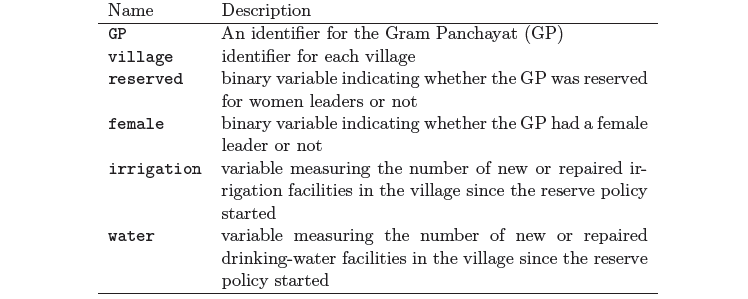
\includegraphics[width=1.1\textwidth]{"C:\\Users\\User\\Desktop\\my_answers\\women_desc.png"}	
\end{figure}		
\newpage
\begin{enumerate}
	\item [(a)] State a null and alternative (two-tailed) hypothesis.
	\newline 
	H0: the reservation policy has no significant effect on the number of new or repaired drinking water facilities in the village \((\beta = 0)\)
	\newline
	H1: the reservation policy has a significant effect on the number of new or repaired drinking water facilities in the village \((\beta \neq 0)\)
	\vspace{0.6cm}
\end{enumerate}
	Run a bivariate regression to test this hypothesis include your code.
	\newline

	now running the bi variate model
	\lstinputlisting[language = R, firstline =115, lastline =121 ]{"C:\\Users\\User\\Desktop\\my_answers\\PS02_R.R"}
	\begin{verbatim}
		Call:
		lm(formula = water ~ reserved, data = df2)
		
		Residuals:
		Min      1Q      Median     3Q     Max 
		-23.991 -14.738  -7.865   2.262 316.009 
		
		Coefficients:
		              Estimate   Std. Error t value  Pr(>|t|)    
		(Intercept)   14.738      2.286   6.446    4.22e-10 ***
		reserved       9.252      3.948   2.344    0.0197 * 
		---
		Signif. codes:  0 ‘***’ 0.001 ‘**’ 0.01 ‘*’ 0.05 ‘.’ 0.1 ‘ ’ 1
		
		Residual standard error: 33.45 on 320 degrees of freedom
		Multiple R-squared:  0.01688,	Adjusted R-squared:  0.0138 
		F-statistic: 5.493 on 1 and 320 DF,  p-value: 0.0197
	\end{verbatim}
	\textbf{p-value}
	\newline
	The p-value for our slope associated with the reservation policy is 0.0197.
	\newline
	\textbf{Conclusion} 
	\newline
	Since this p-value is less than our significance level of 0.05, we conclude that the slope is statistically significant. Therefore, we have sufficient evidence to reject the null hypothesis, which states that there is no relationship between the reservation policy and the number of new or fixed water facilities. This suggests that changes in the reservation policy are associated with changes in the number of water facilities, indicating a significant relationship between these variables.
	\vspace{0.8cm}
	
	Interpret the coefficient estimate for reservation policy
	\begin{itemize}
	\item  the linear regression model indicates that when the reservation policy is at zero the estimated number of new or fixed water facilities is 14.73, moreover, the number of fixed or new water facilities tends to increase by 9.25 for every one unit change in the reservation policy.
	\item also the p-value for the slope(reservation policy) is 0.01 which is less than the significance level of0.05 therefore we can reject the null hypothesis that there exists no relationship between reservation policy and number of water facilities, and the slope estimate of 9.252 did not occur by random chance 
	\item Additionally, the p-value for the slope (reservation policy) is 0.01, which is less than the significance level of 0.05. Therefore, we can reject the null hypothesis that there is no relationship between the reservation policy and the number of water facilities. This suggests that the slope estimate of 9.25 is statistically significant and did not occur by random chance. 
	\item also only 33.45percent of variance in the number of water facilities can be explained by the reservation policy 
	\end{itemize}
	
	
	
	

\end{document}
